% !TeX root = Protokoll.tex
\subsection{Funktionsweise eines Lasers}
\begin{figure}[b!]
	\centering
	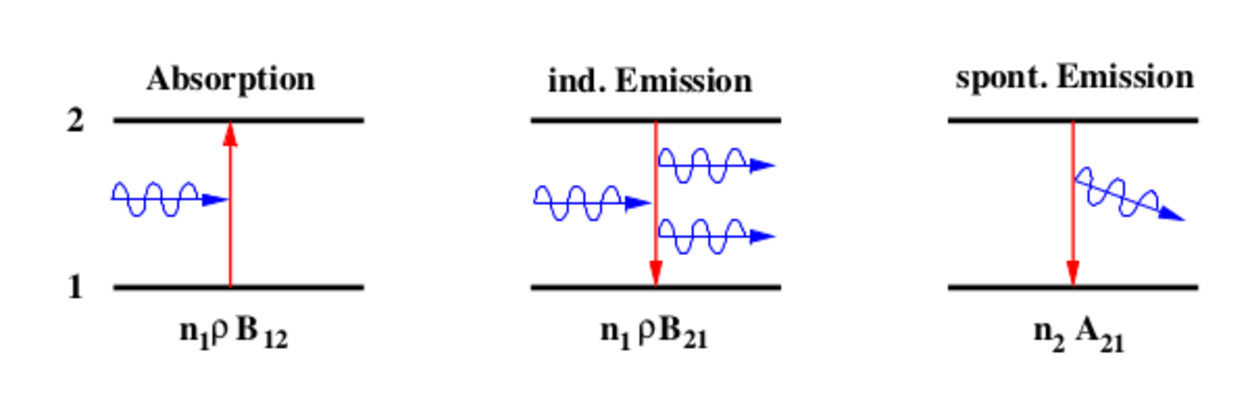
\includegraphics[width = \textwidth]{../Grafiken/Emission.pdf}
	\caption{Hier sind die Emissionen und Absorptionen schematisch dargestellt.\cite{V61}}
\end{figure}
Dieser Abschnitt wurde mithilfe von \cite{V61} erstellt.\\
Grundlegend besteht ein Laser aus drei Komponenten, dem Lasermedium, dem Resonator und einer Pumpquelle.
Die Pumpquelle regt das Lasermedium an, wodurch das Medium Licht emittiert.
Mithilfe des Resonators wird das Licht mehrfach durch das Lasermedium geleitet, wodurch mehr Licht emittiert wird das genau die gleiche Wellenlänge besitzt wie das Licht das es angeregt hat.
Dies hat zur Konsequenz, dass der Laserstrahl hohe Intensität und  Kohärenz besitzt.
Um diesen Prozess genauer zu verstehen, wird das Beispiel eines Zwei-Niveau-Lasers betrachtet.
Durch ein Photon, das die Energie des Übergangs besitzt, geht das System vom Grundzustand (1) in den angeregten Zustand (2) über.
Die Kohärenz wird dabei durch die induzierte Emission erreicht.
Wenn ein Photon auf das System  trifft, wird ein weiteres Photon heraus gelöst, dieses besitzt die selbe Energie, Phase und Ausbreitungsrichtung wie das auslösende Photon.
Dies ist der Effekt der induzierten Emission und der Grund warum Laser so kohärent sind.
Weiter ist es möglich, dass ein Photon durch spontane Emission emittiert wird, dieses Photon besitzt eine beliebige Phase und Ausbreitungsrichtung.\\
Mithilfe eines Strahlenfeldes $\rho$ lassen sich spontane und induzierte Emission hervorrufen.
Dadurch lässt sich für die Photonenanzahl im System die Gleichungen
\begin{align}
	\dot{N}_A=n_1\rho B_{12}\\
	\dot{N}_{IE}=n_2\rho B_{21}\\
	\dot{N}_{SE}=n_2A_{21}
\end{align}
aufstellen. Hier bezeichnet $n_i$ die Besetzungszahl des Niveaus an, $\dot{N}_A$ ist die Änderung der Photonen durch Absorption, $\dot{N}_{IE}$ die Änderung durch induzierte Emission und $\dot{N}_{SE}$ die Änderung durch spontane Emission.
Weiter sind die Konstanten $A_{21},\ B_{12}$ und $B_{21}$ die Einsteinkoeffizienten und geben die Übergangswahrscheinlichkeiten an.
Es lassen sich daraus nun für den Fall, dass die Summe der Besetzungszahlen konstant ist die Gleichungen
\begin{align}
	\frac{dn_1}{dt}=&-n_1\rho B_{12}+n_2\rho B_{21}+n_2A_{21}\\
	\frac{dn_2}{dt}=&+n_1\rho B_{12}- n_2\rho B_{21}-n_2A_{21}
\end{align}
aufstellen.
Damit ein Laser dauerhaft kohärent bleibt, müssen die höheren Niveaus stärker besetzt sein, als das Grundniveau.
Dies wird Besetzungsinversion genannt. 
Das hat zur Folge, dass spontane Emission seltener auftritt als die induzierte  Emission.
Um den Zustand der Besetzungsinversion aufrecht zu erhalten, muss dem System dauerhaft Energie hinzugefügt werden.
Dies wird mithilfe der Pumpquelle gewährleistet.
\subsection{Diodenlaser}
\begin{figure}[h!]
	\centering
	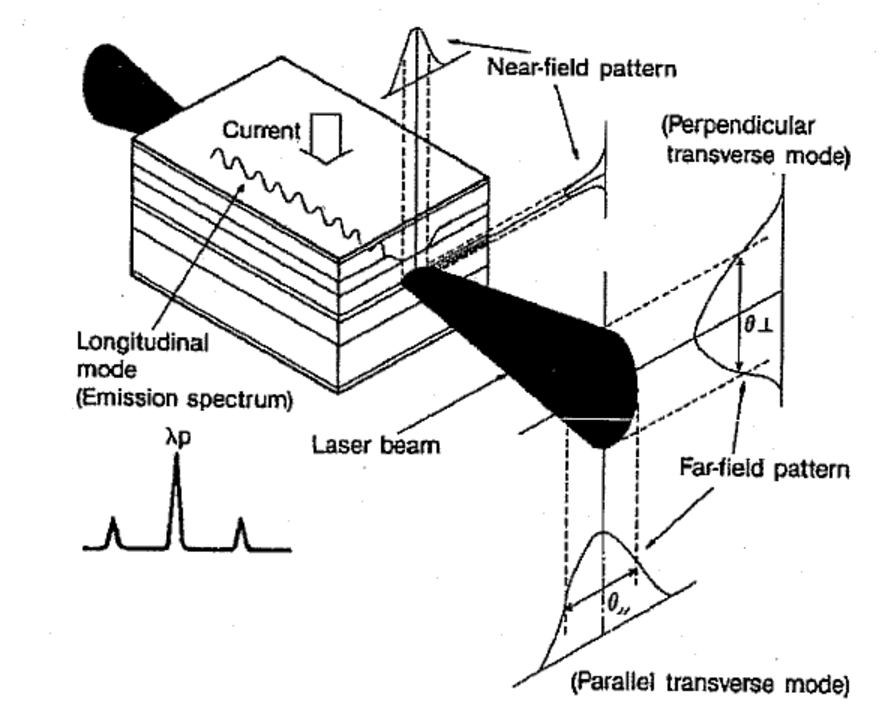
\includegraphics[width = 0.5\textwidth]{../Grafiken/Schematische_Ansicht_Laserdiode.pdf}
	\caption{Skizze des Chips eines Diodenlasers.\cite{V60}\label{fig:Halleiter-Chip}}
\end{figure}
Ein Vorteil des Diodenlasers ist die Bandbreite der abgedeckten Frequenzen $\Delta \nu = \SI{1}{\mega\hertz}$.
Das Lasermedium wird bei einem Diodenlaser mithilfe eines Halbleiters verwirklicht.
Ein LED-Chip, wie er hier verwendet wird, ist in \cref{fig:Halleiter-Chip} skizziert.
Der Strom fließt von oben nach unten, wodurch Elektronen-Loch-Paare erzeugt werden und bei der Rekombination werden Photonen emittiert.
Damit der Chip kohärentes Licht emittiert, muss der Betriebsstrom einen gewissen Wert übersteigen, darunter funktioniert der Halbleiter wie eine normale LED.
Weiter sind die Brechungsindices der aktiven Schicht größer als die der benachbarten Schichten, damit wird der Laserstrahl durch die aktive Schicht geführt.
Die beiden Flächen durch die der Strahl führt sind verspiegelt, wobei die eine Seite fast einfallendes Licht fast vollständig reflektiert und die andere Seite teildurchlässig ist.
Dies bildet den inneren Resonator (internal cavity) und gibt dem Laser eine bevorzugte Richtung.
Da der Strahl allerdings sehr divergent ist, wird noch eine Sammellinse eingebaut.
Nach der Sammellinse wird ein Gitter eingebaut.
Dies sorgt dafür, dass ein großer Teil des gebeugten Lichtes zurück in die Diode strahlt und einen äußeren Resonator bildet (external cavity).
Der Rest bildet den aus gekoppelten Laserstrahl.
Dieser Aufbau ist in \cref{fig:Aufbau_Gitter_Laserdiode} skizziert.
Ein Nachteil des Diodenlasers ist das er anfällig für optisches Feedback ist.
Dies wird durch den Aufbau verhindert.
Ebenfalls wird dadurch ermöglicht die Wellenlänge, auf eine bestimmte Wellenlänge festzulegen.
\begin{figure}
	\centering
	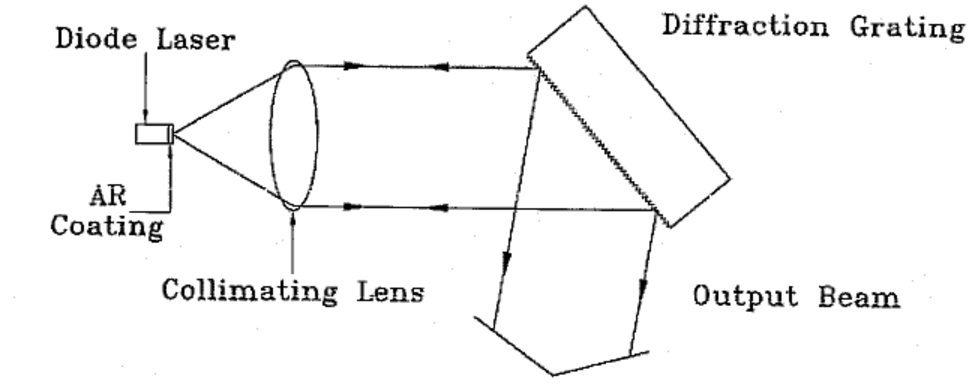
\includegraphics[width = 0.75\textwidth]{../Grafiken/Aufbau_Gitter_Laserdiode.pdf}
	\caption{Hier ist der Aufbau einer Laserdiode mit Gitter skizziert.\cite{V60}\label{fig:Aufbau_Gitter_Laserdiode}}
\end{figure}
\newpage
\subsection{Abstimmen des Lasers}
\begin{figure}[h!]
	\centering
	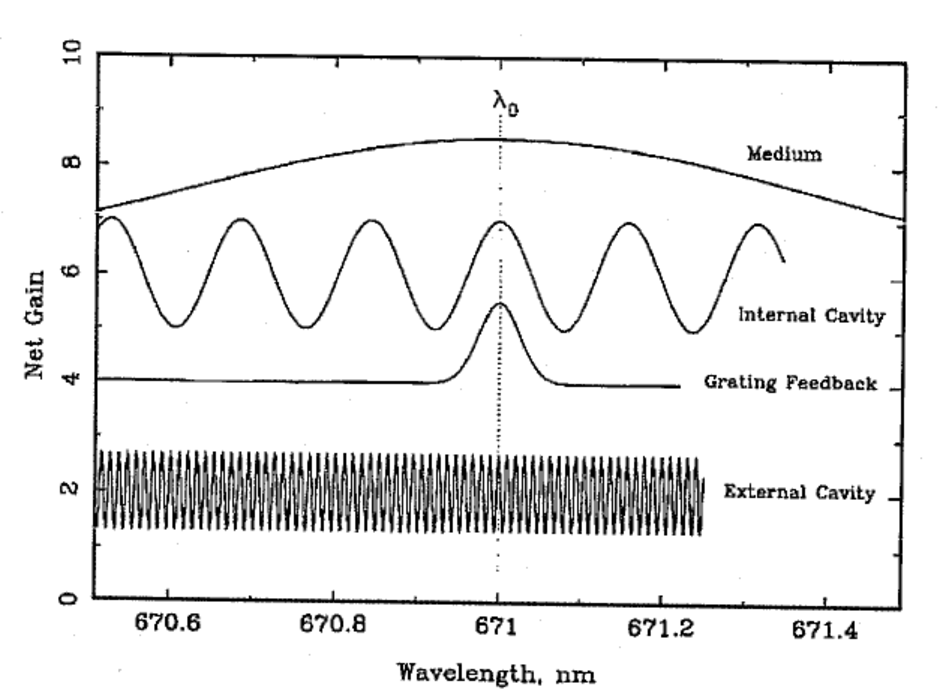
\includegraphics[width = 0.75\textwidth , angle = 1]{../Grafiken/Photon_Gain_Wellenlaenge_Beitraege.pdf}
	\caption{Hier sind die Auswirkungen, der Verschiedenen Effekte auf die Wellenlänge, schematisch dargestellt.\cite{V60}\label{fig:Photon_Gain_Wellenlaenge_Beitraege}}
\end{figure}
Aufgrund der induzierten Emission, emittiert der Laser nur das Licht mit der Wellenlänge, bei der die größte Verstärkung auftritt.
Die Wellenlänge hängt demnach von verschiedenen Effekten ab.
Diese werden im folgenden diskutiert und sind in \cref{fig:Photon_Gain_Wellenlaenge_Beitraege} angedeutet.
\subsubsection{Materialabhängigkeit}
Die Wellenlänge des Materials hängt in erster Linie von der Größe der Bandlücke ab.
Dies ist eine Temperaturabhängige Größe, das heißt sie kann durch erhitzen der Diode eingestellt werden.
Da die hervorgerufene Materialverstärkung sehr Breit ist, muss sie nicht genau auf das Maximum der gewünschten Wellenlänge eingestellt werden.
\subsubsection{Innerer Resonator}
Ein Resonator besitzt verschiedene longitudinale Moden.
Das bedeutet das im Resonator stehende Wellen vorliegen. Die Wellenlängen $\lambda$ dieser stehenden Wellen
erfüllen die Gleichung
\begin{empheq}{equation}
	N\lambda = 2L = 2\frac{L^{\prime}}{n}
\end{empheq}
mit der optischen Weglänge $L^{\prime}$, welche der Strecke entspricht, die Licht im Vakuum in
gleicher Zeit zurücklegt, wie Licht, das sich durch ein Medium der Länge $L$ und mit Brechungsindex
$n$ ausbreitet.
Die Moden des inneren Resonators, hängen dabei vom Betriebsstrom der Diode ab.
Zu einem erhitzt der Strom die Diode.
Dies beeinflusst die Wellenlänge, in dem sich der Resonator ausdehnt und so die Länge $L$ ändert.\\
Zum anderen ändert sich die emittierte Wellenlänge, dadurch das die Ladungsträgerkonzentration steigt.
Der Brechungsindex $n$ ist von der Ladungsträgerkonzentration abhängig.
Dies sorgt dafür, dass sich die optische Weglänge verändert.
\subsubsection{Das Gitter Feedback}
Das Experiment verwendet die Littrow-Anordnung.
Dabei wird das erste Beugungsmaximum zurück in in den Diodenlaser geleitet.
Wobei die Bragg-Bedingung gilt
\begin{align}
	\lambda = 2d\sin\theta.
\end{align}
Hier ist $d$ der Gitterabstand und $\theta$ der Gitterwinkel.
\subsubsection{Äußerer Resonator}
Die Einflüsse des äußeren Resonators ähneln dem inneren. 
Dadurch das der äußere Resonator so viel größer ist als der innere, liegen die Maxima der longitudinalen Moden enger zusammen.
Durch ändern der Position des Gitters ändert sich die Länge des äußeren Resonators und somit die Form der Moden.
\subsection{Modensprünge}
Modensprünge treten auf wenn einer der beiden Resonatoren verstellt wird.
Da allerdings das Ziel des Versuches ist eine kontinuierliches Wellenlängenspektrum zu erzeugen, um damit das Absorptionsspektrum von Rubidium untersuchen zu können, müssen diese verhindert werden.
Dazu wird erst ein mal der Ursprung dieser Modensprünge verdeutlicht. 
\begin{figure}[h!]
	\centering
	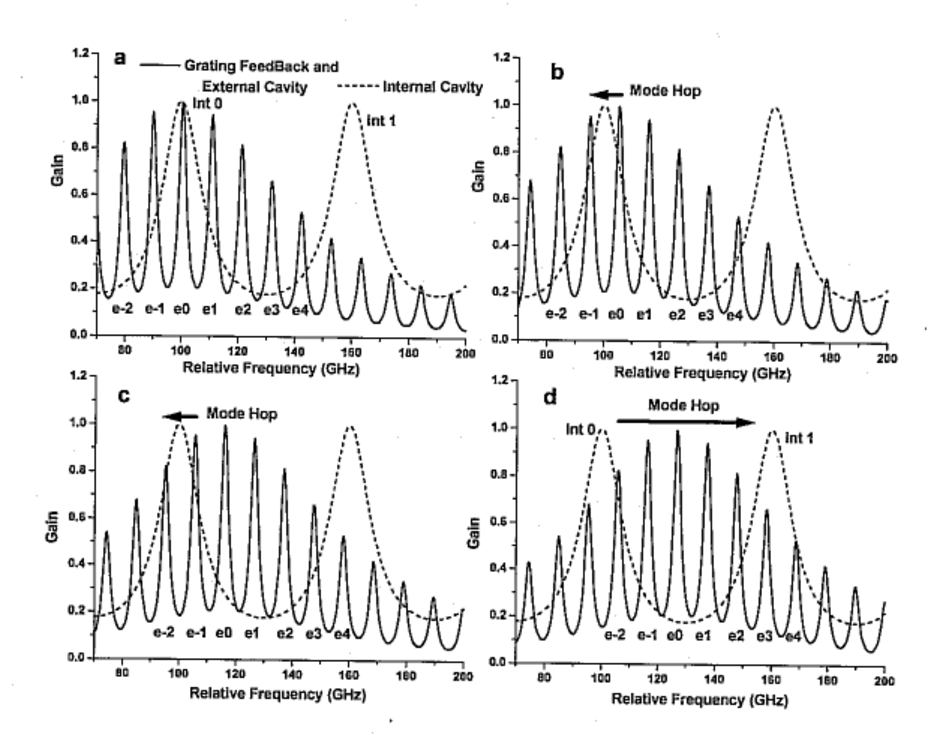
\includegraphics[width = 0.75\textwidth, angle = 1]{../Grafiken/Moden_Spruenge.pdf}
	\caption{Hier ist die Kombination des Gitter Feedback und des Äußeren Resonators sowie extra der innere Resonator für verschiedene Winkel dargestellt.\cite{V60}\label{fig:Moden_Spruenge}}
\end{figure}
In \cref{fig:Moden_Spruenge} ist eine Kombination des äußeren Resonator und des Gitter Feedbacks sowie der innere Resonator eingezeichnet.
Von Bild a bis zu Bild d wird der Gitterwinkel immer weiter verringert.
In Bild a ist der Winkel so eingestellt, dass das Maximum e0 der äußeren Einflüsse auf dem Maximum Int0 des inneren Resonators liegt.
Die komplette Verstärkung hängt von beiden Linien ab.
Dies bedeutet, dass in Abbildung b Modensprünge auftreten.
Das heißt die Mode springt vom Maximum e0 zu Maximum e-1.
In c springt es von e-1 nach e-2.
Während der Winkel immer kleiner wird springt in die Mode ins Maximum e3.\\
Es ist nötig diese Sprünge zu verhindern, um ein vollständiges Wellenlängenspektrum zu verwirklichen.
Dies kann verhindert werden in dem ebenfalls der innere Resonator angepasst wird.
Bedeutet man verstellt den Winkel und den Betriebsstrom der Diode gleichermaßen.